\section{\textbf{Proposed Suspicious Text Detector}}
The key objective of our project is to design a system that can classify suspicious and non-suspicious text. \textbf{Fig} \ref{fig:proposed_model} shows an abstract view of our suspicious text detector classifier.

\begin{figure}[h!]
\centering
  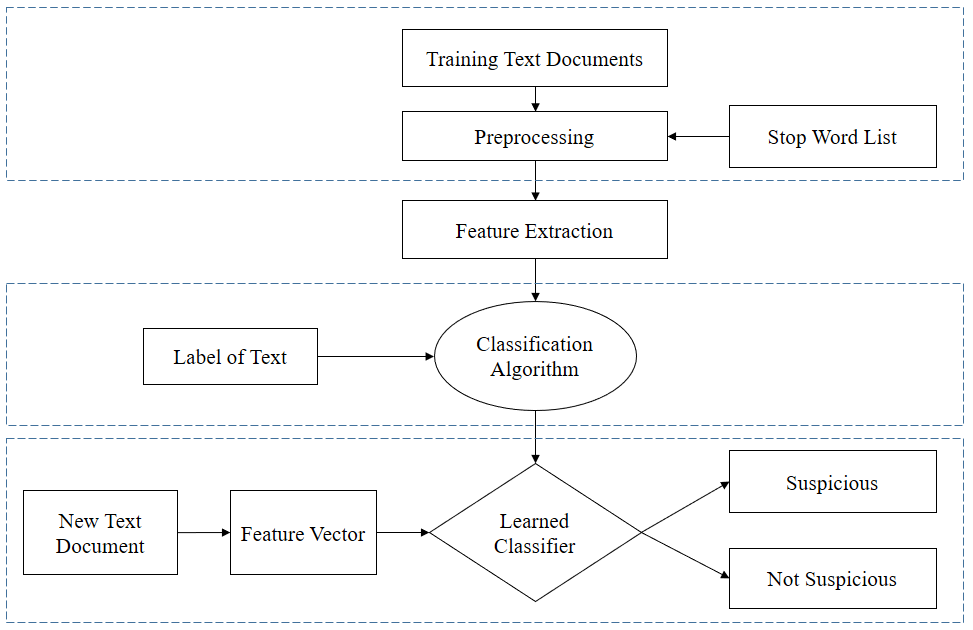
\includegraphics[height=6.8cm, width=8.8cm]{Figures/pr_model.PNG}
  \caption{ Suspicious Text Detection Model}
  \label{fig:proposed_model}
\end{figure}

We have tested this system by using different supervised machine learning algorithms. Our whole model is divided into four different phases.
\subsection{\textbf {Training Set Preparation}}
Our training set $T = \{t_1, t_2, t_3, ..., t_n\}$ consists of $n$ training text documents. Each text is labeled as either suspicious or non suspicious. Suspicious class is denoted by $C_s$ and non suspicious class is denoted by $C_{ns}$.\par
A random text $t_i$ with $k$ words is represented by a word vector $W[] =\{w_1, w_2, w_3, ....., w_k\}$ in our system,
\begin{table}[h!]
\begin{center}
\caption{Word representation of a text}
\begin{tabular}{|m{1cm} | m{1cm}| m{1cm}|m{1cm} | m{1cm}|}
\hline
     $w_1$ & $w_2$  & $w_3$ & $...$ & $w_k$  \\
\hline
\end{tabular}
\end{center}
\end{table}

All texts are preprocessed by the preprocessor in order to remove inconsistencies from dataset. We have developed a list $S[]=\{s_1, s_2, s_3, ..., s_r\}$ with $r$ stop words which is a column vector where each row contains a stop word.\par
\begin{figure}[h!]
    \centering
    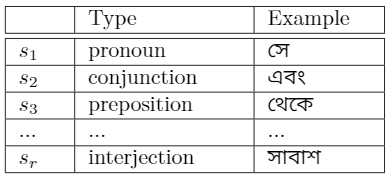
\includegraphics[width=7cm,height=3.8cm]{Figures/stop.PNG}
    \caption{Stop word list}
    \label{fig:ss}
\end{figure}
\vspace{0.1cm}
In our system the word $w_i$ which has no contribution in deciding whether a text $t_i$ is suspicious ($C_s$) or not suspicious $(C_{ns})$ is referred as stop word $s_i$. Pronoun, conjunction, preposition, interjection, prefix and suffix are considered as stop words. Stop words $ s_1, s_2, s_3, ..., s_r$ are removed form the text $t_i$ by matching with the stop word list $S[]$. Punctuation's in a text are also removed in preprocessing step.

\subsection{\textbf{Feature Extraction}}
A word list is created by the tokenizer by tokenizing the main body of a text. Word frequencies are used as features in this system. Bag of words model is used to represent the features.
\renewcommand{\arraystretch}{1.3}
\begin{table}[h!]
\begin{center}
\caption{A small fragment of feature space}
\begin{tabular}{|m{0.7cm} || m{0.7cm}| m{0.7cm}|m{0.7cm} | m{0.7cm}|m{1cm}|m{0.7cm}|}
\hline
  \backslashbox{r}{c} & $w_1$ & $w_2$  & $w_3$ &$w_4$ &$...$ & $w_j$  \\
\hline
\hline
     $t_1$ & $2$ & $0$  & $0$ &$4$ &$...$ & $1$  \\
\hline
     $t_2$ & $0$ & $0$  & $1$ &$0$ &$...$ & $5$  \\
\hline
     $t_3$ & $4$ & $0$  & $2$ &$2$ &$...$ & $0$  \\
\hline
     $t_4$ & $0$ & $3$  & $0$ &$0$ &$...$ & $2$  \\
\hline
     $...$ & $...$ & ...  & $...$ &$...$ &$...$ & $...$  \\
\hline
     $t_i$ & $0$ & $0$  & $3$ &$1$ &$...$ & $0$  \\
\hline
\end{tabular}
\label{ff}
\end{center}
\end{table}
Table \ref{ff} shows the feature space for our system. Our feature space ($F[][]$) is a two dimensional ($i\times j$) array with $i$ rows and $j$ columns.
Here rows represents the texts $t_1, t_2, t_3, ..., t_i$ available in the corpus and columns represents total number of unique words $w_1, w_2, w_3, ....., w_j$ in the corpus. The value of $i$ is $1500$ and value of $j$ is $3250$ respectively as we have $1500$ text document and $3250$ unique words in our training set $T$. Each cell of the array represents the frequency ($f_{ij}$) of a specific word $w_j$ occurs in a specific text $t_i$. Each row of the feature matrix represents features $F[][] =\{F[1], F[2], F[3], ... ,F[n]\} $ for the texts of the dataset. 

\subsection{\textbf{Classification Algorithm}}
It is the most important part of our whole system. By using extracted features $F[1], F[2], F[3], ... ,F[n]$ and applying a suitable learning algorithm we train our model to classify texts as suspicious $C_s$ and non suspicious $C_{ns}$. Mainly logistic regression is used to implement the system and other algorithms are applied to establish comparison. 
\vspace{0.3cm}

\textbf{Logistic Regression} \cite{sharma2015active} is a binary classification model that predicts a binary outcome based on some features. The output of logistic regression depends on logistic function. The logistic function is a sigmoid function, which takes any real input and outputs a value between zero and one.This function ensures the output of our model does not become less than zero and greater than one. The definition of logistic function or hypothesis function is,
\begin{equation}
    h_{\theta}(x) =  \frac{1}{1+\exp({-\theta^T x})}
\end{equation}
Cost function for Logistic regression is,
\begin{equation}
    J(\theta) = \frac{1}{m}\sum_{i-1}^{m}cost(h_{\theta}(x^{i}),y^{i})   
\end{equation}

\[
cost(h_{\theta}(x), y) = 
\begin{cases}
    -\log (h_{\theta}(x)) & \texttt{if } y = 1\\
     -\log (1-h_{\theta}(x)) & \texttt{if } y = 0
\end{cases}
\]
Here,\\
$m = $ Number of training examples.\\
$h_{\theta}(x^{i}) = $ Hypothesis function of $i_{th}$ training example\\
$y^i = $ Input label of $i_{th}$ training example.
\vspace{0.2cm}

\noindent
Writting the cost function in this way guarantees that $J(\theta)$ is convex for logistic regression.
%\vspace{0.1cm}
%\par
For binary logistic regression selecting
the threshold value is an important task, everything below threshold will be considered as 0 or negative otherwise it will be 1 or positive.


\vspace{0.3cm}
\textbf{Naive Bayes} \cite{yoo2015classification} can be defined as Bayes theorem with a conditional independency assumption that all variables $A_{1},A_{2},...,A_{n}$ in a given category $C$ are conditionally independent with each other given $C$. 
According to Bayes rule for a text document $(T)$ and class $(C)$ we can write,
\begin{equation}
    P(C|T) = \frac{P(T|C)P(C)}{P(T)}
\end{equation}
Final equation for Naive Bayes classifier is,
\begin{equation}
     C_{MAP} = argmax P(X_{1},X_{2},...,X_{n}|C)P(C)
\end{equation}

%\vspace{0.2cm}
we also use support vector machine, k-nearest neighbour and decision tree as classification algorithm to test proposed system. The result of training phase is used in testing phase. This result is saved as a model $(M)$ which classifies a new text document $(t)$ into suspicious $(C_s)$ and non suspicious $(C_{ns})$ category. 
\subsection{\textbf{Testing Phase}}
Testing is the most important phase for any machine learning model. Classification accuracy of the text classifier is calculated in testing phase. In our system testing phase is quite similar as training phase but in this part our learned classifier model is used for predicting. A test set $TS =\{ts_1, ts_2, ts_3, ..., ts_l\}$ is built to test the system which has $l$ text document. Sample texts are taken to test the system. After processing, using feature extraction methods features ($F[][]=\{F[1], F[2], F[3], ... ,F[l]\}$) are extracted from the testing texts $ts_1, ts_2, ts_3, ..., ts_l$. Our trained classifier model use this features to classify a text $ts_i$ as suspicious ($C_s$) and non suspicious ($C_{ns}$).